%%% This file contains the first  report. It cannot be compiled on it's own.

%{{{
\setcounter{section}{1}
%\section{Versuch 1}
\addsec{Versuch 1}
%{{{
In diesem Versuch ging es darum, ein wenig Löterfahrung zu sammeln, das Netzteil und das Multimeter kennen zu lernen und ein paar Messungne bei Gleichstrom durchzuführen.
Bevor die eigentlichen Versuche losgehen konnten, bekamen wir zuerst die Werkzeuge, die wir zur Durchführung der Versuche benötigen. Die Wichtigsten darunter waren, die Platine, auf die die meisten Versuche aufgebaut werden, sowie die nötigen Messkabel und Lötwerkzeuge.
%}}}

%{{{
\subsection{Ohm'sches Gesetz}
In diesem Versuch wird das Ohm'sche Gesetz an einem Widerstand nachgemessen.
Das Skript schlägt 2 verschiedene Möglichkeiten vor, wie die Messgeräte platziert werden könnten:
\begin{figure}[H] %% There is no sense in having this image appear somewhere else
	\centering
	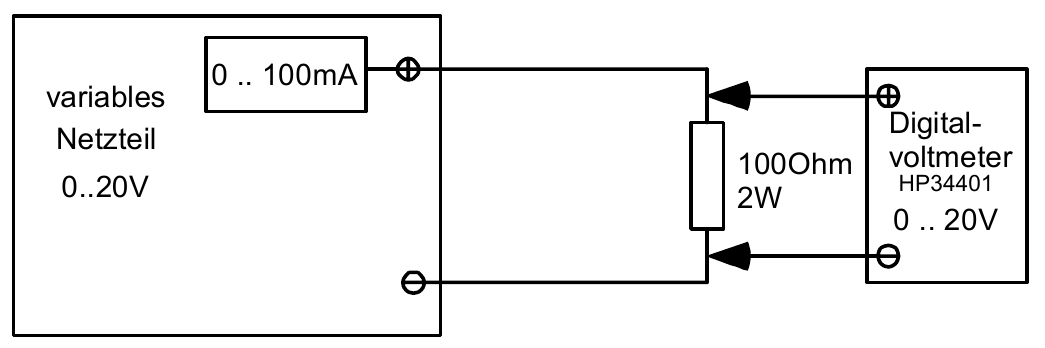
\includegraphics[width=\linewidth]{versuch1/v1_1_Schaltungsvorschlag1}
	\caption{Schaltungsvorschlag 1 aus der Praktikumsanleitung}
\end{figure}
In dieser Schaltung ist das Voltmeter parallel zum zu vermessenden Widerstand geschalten. Dadurch addiert sich sein innerer Leitwert zu dem des Widerstandes und trägt so zum vom Netzteil gemessenen Strom bei. Dieser Effekt ist einer der Gründe, warum man versucht, Voltmeter mit möglichst hohem Innenwiderstand zu bauen, sodass ihr Leitwert im Vergleich mit dem Widerstand nicht ins Gewicht fällt.
Unser Testwiderstand hat 100\Omega bei einer Genauigkeit von 1\%.
Das Multimeter, das wir verwenden, das Agilent HP34401, besitzt in dieser Kombination einen Eingangswiderstand von 10M\Omega \cite{hp34401}. Sein Leitwert ist also $\frac{1}{100000}$ dessen des Testwiderstandes. Damit ist der Messfehler, den wir durch das Multimeter einführen, um einen Faktor 1000 kleiner als die Toleranz des Testwiderstandes.

\begin{figure}[H] %% There is no sense in having this image appear somewhere else
	\centering
	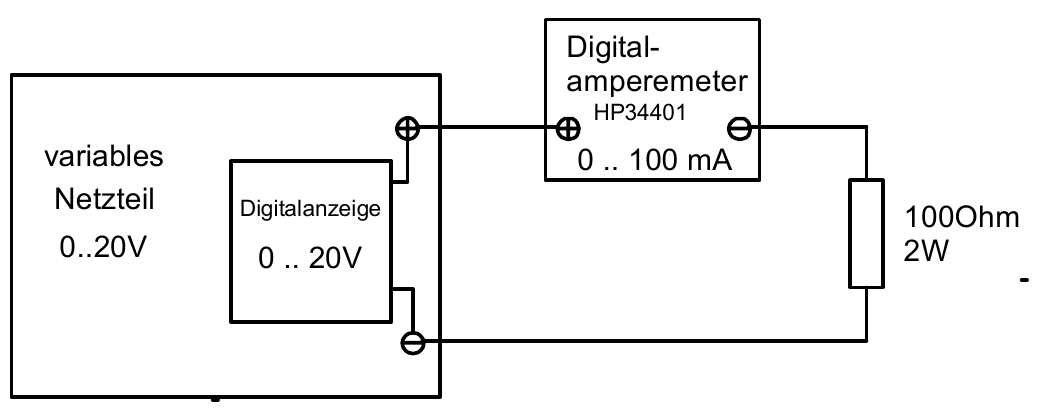
\includegraphics[width=\linewidth]{versuch1/v1_1_Schaltungsvorschlag2}
	\caption{Schaltungsvorschlag 2 aus der Praktikumsanleitung}
\end{figure}
Bei diesem Vorschlag ist das Multimeter als Amperemeter in Serie zum Widerstand geschalten; die Spannung wird durch das im Netzteil integrierte Voltmeter gemessen. Auch hierbei tritt ein der Messgenauigkeit abträglicher Effekt ein: Der Widerstand des Amperemeters und der zuführenden Kabel addiert sich zu unserem Testwiderstand.
Falls der so zugefügte Widerstand gering ist, also $R(Amperemeter) \ll R(Widerstand)$, so fällt dieser nicht mehr ins Gewicht, weil er kleiner als die Toleranz wird. Leider ist der Innenwiderstand des Amperemeters in dem Bereich, in dem wir messen wollen, nicht viel kleiner, als unser Testwiderstand.
Da wir jedoch den Widerstand des Amperemeters kennen, und mit guter Näherung davon ausgehen können, dass die Kabel einen vernachlässigbaren Anteil zum Gesammtwiderstand beitragen, könnten wie den Effekt aus dem Ergebnis wieder herausrechnen.

Der Schaltplan zum auf der Platine verwendeten Aufbau ist:
\begin{figure}[H] %% There is no sense in having this image appear somewhere else
	\centering
	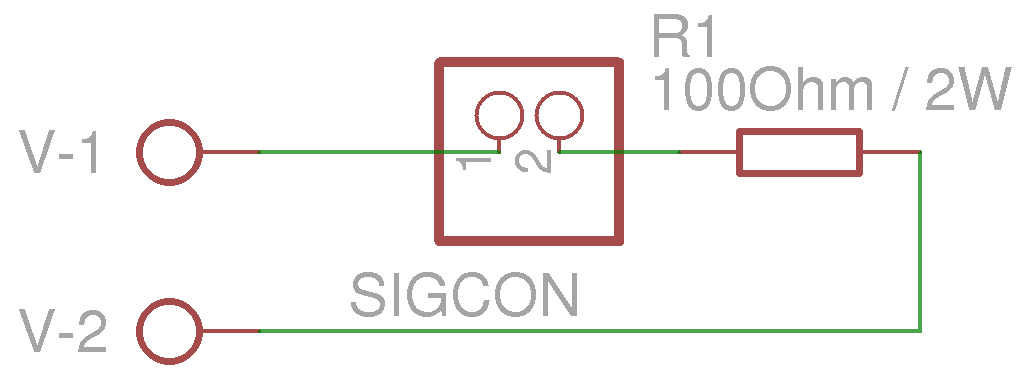
\includegraphics[width=\linewidth]{versuch1/versuch1_schaltplan}
	\caption{Schaltplan zu Schaltungsvorschlag 1}
\end{figure}

In unserem Versuch habe ich den 2. Schaltungsvorschlag verwendet und damit folgende Kennlinie aufgenommen:
\begin{figure}[H] %% There is no sense in having this image appear somewhere else
	\centering
	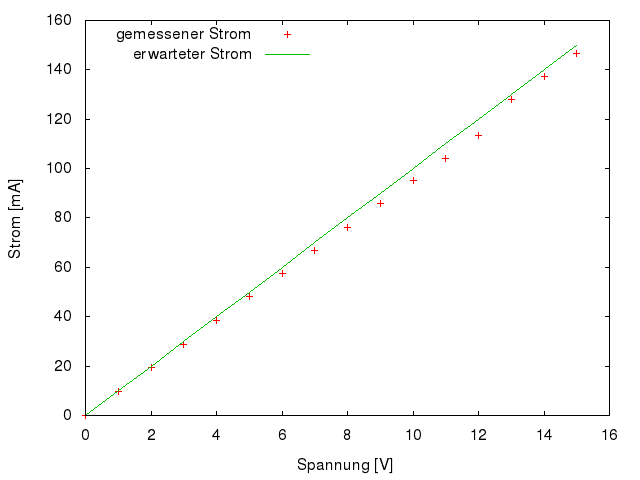
\includegraphics[width=\linewidth]{versuch1/versuch_1_1}
	\caption{Strommessung am 100\Omega-Widerstand}
\end{figure}
Hier sieht man bis 12 Volt schön die gerade Kennlinie, die man für ein lineares Bauteil wie einen einfachen Widerstand erwarten würde. Allerdings zeigt sich hier der zusätzliche Widerstand des Amperemeters, wodurch die Linie gegenüber der erwarteten Linie verflacht ist.
Ausserdem zeigen sich bei 12 und 13 V 2 Knicke in der Kurve. Diese stammen nicht vom Widerstand (der sich weiterhin linear verhält), sondern vom Amperemeter. Dessen Innenwiderstand veringert sich nämlich an dieser Stelle von 5\Omega auf 0.5\Omega. Durch den verringerten Gesammtwiderstand steigt der Strom pro Volt an und bei den nächsten Messungen (ab 13V) zeigen sich die größeren, näher an der Erwartung liegenden Werte.
Die Verlustleistung des Widerstandes in meinem Aufbau bei 15V beträgt also $P_{Verlust} = 15V * 146.500mA = 2197.5 mW \approx 2.2W$,
der größte Fehler bei 6.7mV $\stackrel{\wedge}{=}$ 0.059\%.

Generell scheint mir der erste Aufbau mit den uns gegebenen Größen also günstiger, da der Messfehler hier zum einen deutlich kleiner als die Toleranz ist, und zum anderen keine Messbereichsumschaltungen während der Messung nötig sind.
%}}}

%{{{
\subsection{Kennlinie einer Glühlampe}
In diesem Versuch sollte die Kennlinie eines nichtlinearen Bauteils, nämlich einer Glühlampe ermittelt werden.
Hierzu ist es sinnvoll, zur Spannungsmessung direkt die Anzeige im Netzteil zu verwenden, und den Strom mit dem Multimeter zu messen, da der Strom der Glühlampe die eigentliche Messgröße ist, und wir ausserdem das Labornetzteil als Spannungsquelle verwenden, sodass wir im Netzteil eben auch gerade das anzeigen lassen, was das Netzteil tut.
Die aufgenommene Kennlinie sieht wie folgt aus:
\begin{figure}[H] %% There is no sense in having this image appear somewhere else
	\centering
	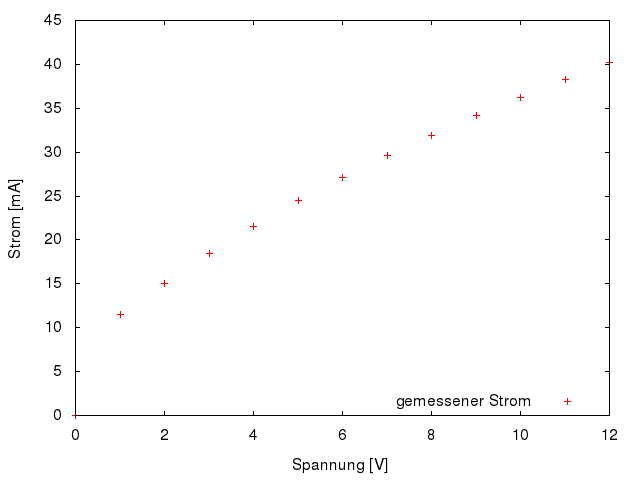
\includegraphics[width=\linewidth]{versuch1/versuch_1_2}
	\caption{Strommessung an einer 12V/40mA-Glühlampe}
\end{figure}
Die Nichtlinearität der Lampe zeigt sich deutlich in der Kennlinie. Die Nichtlinearität rührt daher, dass Metalle im allgemeinen einen positiven Temperaturkoeffizienten haben und sich somit bei steigender Temperatur ihr Widerstand ehöht. Da bei Glühlampen die Drahtwendel buchstäblich glüht, zeigt sich der Effekt sehr ausgeprägt.
%}}}

%{{{
\subsection{Spannungsteiler}
In diesem Versuch wurde ein einfacher Spannungsteiler aus 2 10k\Omega-Widerständen aufgebaut und ausgemessen.\\
$U_L=U_{Aus}=7.4773V,\; I_{Kurzschluss}=1.4995mA$\\\\
$\Rightarrow R_i = \frac{U_{Leerlauf}}{I_{Kurzschluss}} = 1.0003*10^{4}\Omega$\\\\
Bei einer idealen Spannungs- oder Stromquelle sollte der Innenwiderstand 0\Omega sein.
%}}}

%{{{
\subsection{Messen großer Ströme oder kleiner Widerstände}
In diesem Versuch wurde der Spannungsabfall eines Lastwiderstandes einmal an der Stromquelle und einmal direkt am Widerstand gemessen.\\\\
\emph{\textbf{Messung direkt am Widerstand:}}\\
$U_{Netzteil}=1.0V,\; I_{Netzteil}=0.915A,\; U_{Widerstand}: 0.95868V \Rightarrow R=\frac{U_{Widerstand}}{I_{Netzteil}}=1.0477$\\\\
\emph{\textbf{Messung am Netzteil:}}\\
$U_{Netzteil}=1.0V,\; I_{Netzteil}=0.928A,\; U_{Widerstand}: 0.99647V \Rightarrow R=\frac{U_{Widerstand}}{I_{Netzteil}}=1.0890$\\\\
Der Einfluss der Messkabel berechnet sich wie folgt:\\\\
$\delta_{U\_Widerstand}=0.99647V-0.95868V=0.037790V$\\\\
$\Rightarrow Fehler=\frac{\delta_{U\_Widerstand} }{0.95868V}=0.039419 \stackrel{\wedge}{=} 3.9419\%$
%}}}

%}}}
